% Homework #3
% COSC552 HCI
%
% Byron Heads
% E00062946

\documentclass[12pt]{article}

\usepackage{graphics}
\usepackage{hyperref}

\title{Homework Set 3 \\
    COSC552 HCI}
\author{ Byron Heads \\
    E00062946 }
\date{\today}

\begin{document}
\maketitle

\section*{A}
\resizebox{\columnwidth}{!}{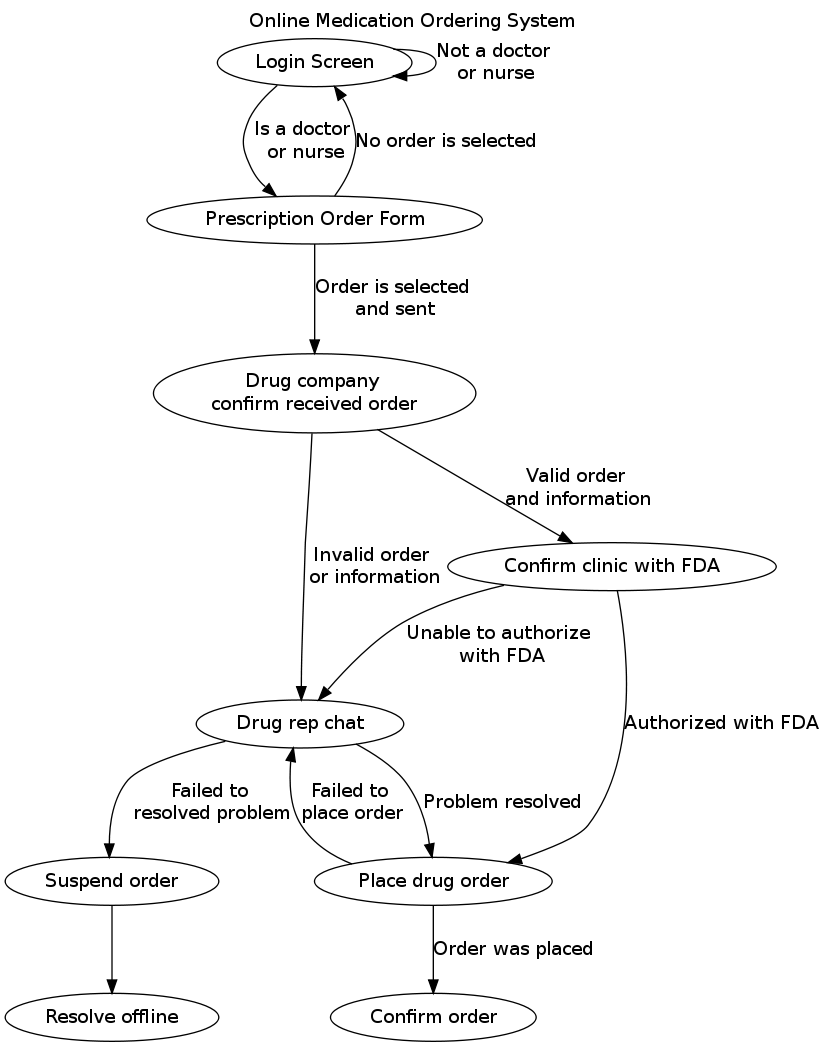
\includegraphics{hw3.png}}

\section*{B}

Training new doctors and nurses on the system can be done through a 
series of collaborative technology.  The first is through a training mode,
this is similar to demos or tutorials found in video games.  The training
mode runs the user step by step through the process of placing fake orders.
The training mode controls the flow of the learning process, and includes 
having the user make mistakes and then fixing them.  The training mode 
asks the user questions during and after different scenarios.  The user is
allowed to email or ask other staff members for answers.

Other technologies such as instant messaging can be deployed to allow staff
members to communicate questions and answers on the use of the system.
Free services such as Google Talk (\url{http://google.com/talk}) can be 
used with open source software like Pidgin (\url{http://pidgin.im}) to 
create an encrypted communication between two or more staff
members.  This technology can be used for free and with encryption can be
safe.  This technology can also be used for video chatting between staff
members.

Other tools such as TightVNC (\url{http://www.tightvnc.com}) can be used to
allow another staff member take control over another computer.  This can be
used to allow another staff member walk another staff member through the
process of using the interface.  This software is available for free, there
are other commercial version of this software as well.

\end{document}

